\documentclass[10pt,a4paper]{report}
\usepackage[utf8]{inputenc}
\usepackage{amsmath}
\usepackage{amsfonts}
\usepackage{amssymb}
\usepackage{graphicx}
\usepackage[final]{pdfpages}
\usepackage{stmaryrd}
\begin{document}

\title{Summary Program Analysis - Spring 2015 ETHZ}
\author{Flurin Rindisbacher}

\maketitle

\tableofcontents

\chapter{Abstract interpretation}
A.I. - invented in late 70s by Patrick Cousot. \\
Frameworks for building analyzers: LLVM, Soot, WALA

\section{Recipe for building a static analyzer}
\begin{enumerate}
 \item come up with an \textbf{abstract domain} (select based on the poperties to prove)
 \item define abstract semantics \textbf{for the programming language} w.r.t. to the abstract domain (define the \textbf{abstract transformer}, the effect of statement/expression on the abstract domain).
 \item iterate until fixed point is reached
\end{enumerate}

\textbf{fixed point} is an \textbf{over-approximation} of the program

\section{Partially Ordered Sets (posets)}
\begin{itemize}
 \item Binary relation $\sqsubseteq$ on a set L (subset of $L \times L$)
 \item \textbf{three properties}: reflexive, transitive, anti-symmetric
 \item Reflexive: $\forall p . p \sqsubseteq p$
 \item Transitive: $\forall {p,q,r} \in L . (p \sqsubseteq q \land q \sqsubseteq r) \implies p \sqsubseteq r$
 \item Anti-symmetric: $\forall p,q . (p \sqsubseteq q \land q \sqsubseteq p) \implies p = q$

\item A poset $(L, \sqsubseteq)$ is a set $L$ equipped with a partial ordering $\sqsubseteq$.
\item $p \sqsubseteq q$ intuitively means, that $p \implies q$ \\
if $p \sqsubseteq q$ then p is "\textbf{more precise}" than q (p represents fewer concrete states than q)

\item \textbf{Least} element ($\bot$) in Poset: $\forall p . \bot \sqsubseteq p$ \\ 
\textbf{Greatest} element ($\top$) in Poset: $\forall p . p \sqsubseteq \top$ \\ **may not exist**. but are unique if they do.
\item $u \in L$ is an \textbf{upper bound} of $Y \subseteq L$ if $\forall p \in Y . p \sqsubseteq u$
\item $l \in L$ is a \textbf{lower bound} of Y if $\forall p . l \sqsubseteq p$
\item $\sqcup Y \in L$ is a \textbf{least upper bound} of Y if $\sqcup Y$ is an upper bound of Y and $\sqcup Y \sqsubseteq u$ whenever $u$ is another upper bound of Y.
\item $\sqcap Y \in L$ is \textbf{greatest lower bound} of Y if $\sqcap Y$ is a lower bound of Y and $\sqcap Y \sqsupseteq l$ whenever l is another lower bound of Y.
\item $\sqcup Y$ and $\sqcap Y$ need not be in Y
\item $p \sqcup q$ and $\sqcup\{p,q\}$ are the same
\end{itemize}
\section{Complete Lattices}
$(L,\sqsubseteq,\sqcup)$ is a poset where $\sqcup Y$ and $\sqcap Y$ exist for any $Y \subseteq L$
\section{Chains}
Given a poset $(L,\sqsubseteq)$, a subset $Y \subseteq L$ is a \textbf{chain} if every two elements in $Y$ are comparable (ordered) \\
$\forall {x,y} \in Y . (x \sqsubseteq y) \lor (y \sqsubseteq x)$
The \textbf{height} of a poset is the chain with the largest size.

\section{Functions}
Let $f: A \to B$, $g: A \to A$, $(A, \sqsubseteq)$ a poset and $x \in A$
\begin{itemize}
\item \textbf{monotone}: \\ 
$\forall a,b \in A: a \sqsubseteq b \implies f(a) \leq f(b)	$ \\
$\forall a,b \in A: a \sqsubseteq b \implies g(a) \sqsubseteq g(b)$
\item \textbf{Fixed Points} \\
x is fixed point iff g(x) = x \\
x is a \textbf{post-fixedpoint} iff $g(x) \sqsubseteq x$ \\
Fix(f) is the set of all fixed points \\
Red(f) = set of all post-fixedpoints \\
\textbf{least} fixed point ($lfp^{\sqsubseteq}f \in L$): is fixed point and all other fixed points are above ($\sqsubseteq$) \\ 
a \textbf{least fixed point may not exist} \\
When does a list fixed point exist? see Tarski's fixed point theorem \ref{Tarski}
\item \textbf{Function iterates}: $g^0(a), g^1(a), g^2(a)$ where $g^{n+1}(a) = g(g^n(a))$ we usually take $a=\bot$
\item \textbf{completely meet-preserving}: for \underline{any subset} $Y \subseteq A$: $f(\sqcap_2 Y) = \sqcap_1\{f(y)|y \in Y\}$ (when $\sqcap_1$ and $\sqcap_2$ exists)
\item \textbf{completely join-preserving}: for \underline{any subset} $Y \subseteq A$: $f(\sqcup_1 Y) = \sqcup_2\{f(y)|y \in Y\}$ (when $\sqcup_1$ and $\sqcup_2$ exists) Sheets 36,37 for examples
\item join-preserving implies monotonity 
\end{itemize}

\subsection{Tarski's fixed point theorem}
\label{Tarski}
if $(L,\sqsubseteq,\sqcup,\sqcap,\bot,\top)$ is \textbf{complete lattice} and \\ $f: L \to L$ is a \textbf{monotone function} \\
then: \\
$lfp^{\sqsubseteq}f$ exists, and \\
$lfp^{\sqsubseteq}f = \sqcap Red(f) \in Fix(f)$

\subsection{iterative algo for fixed point}
\label{fixedpoint_theorem}
Given a poset of \underline{finite} height, a least element $\bot$ and a \underline{monotone} f:\\
The iterates $f^0(\bot), f^1(\bot)..$ form an increasing sequence which eventually stabilizes from some $n \in N$. \\
$f^n(\bot) = f^{n+1}(\bot)$ and: \\
\begin{equation}
\label{eq:iterative_lfp}
lfp^{\sqsubseteq}f = f^n(\bot)
\end{equation}
Equation \ref{eq:iterative_lfp} leads to a simple iterative algorithm for computing $lftp^{\sqsubseteq}f$.

\section{Galois Connection}
Let $(L_1,\sqsubseteq_1,\sqcup_1,\sqcap_1)$ and let $(L_2,\sqsubseteq_2,\sqcup_2,\sqcap_2)$ be complete lattices. \\
Let $\alpha: L_1 \to L_2$ and let $\gamma: L_2 \to L_1$
Then $\alpha$ and $\gamma$ form a \textbf{Galois connection} if:
\begin{itemize}
\item $\alpha$ is monotone
\item $\gamma$ is monotone
\item $\alpha \circ \gamma$ is \underline{reductive}: $\forall x_2 \in L_2: \alpha(\gamma(x_2)) \sqsubseteq_2 x_2$
\item $\gamma \circ \alpha$ is \underline{extensive}: $\forall x_1 \in L_1: \gamma(\alpha(x_1)) \sqsupseteq_1 x_1$
\end{itemize}
Equivalent definition (more useful for proofs):
\begin{equation}
\label{eq:galois}
\forall x_1 \in L_1, \forall x_2 \in L_2: \alpha(x_1) \sqsubseteq_2 x_2 \iff x_1 \sqsubseteq_1 \gamma(x_2)
\end{equation}
\textbf{Intuition}: $\alpha$ and $\gamma$ are monotone because relationshop between information and concrete is \underline{preserved} in the abstract and vice versa. \\
\textbf{Intuition 2}: $\gamma \circ \alpha$ is extensive because $\alpha$ is indeed a correct approximation. \\ \\
Latticed defined over $L_1$ captures the \textbf{concrete}. The other one captures the \textbf{abstract}. $\alpha$ is an \textbf{abstraction function} and $\gamma$ is a \textbf{concretization function}. The galois connections links concrete and abstract.
\subsection{Galois Insertion}
Galois insertion is a Galoise connection where $\gamma$ is also \underline{injective}. This means, that $\alpha \circ \gamma$ is the \underline{identity} function and that $\alpha$ is also \underline{surjective}.\\
\textbf{Intuition}: Each abstract element has a \underline{unique} representation in the concrete.
\subsection{Key property of Galois connection}
The abstraction function $\alpha$ \underline{uniquely determines} the concretization function $\gamma$ and vice versa.\\
\begin{equation}
\label{eq:galois_key_property}
\begin{split}
\underline{if}: (L_1,\sqsubseteq_1,\sqcup_1,\sqcap_1) {}_{\to_{\alpha}}^ {\gets^{\gamma}} (L_2,\sqsubseteq_2,\sqcup_2,\sqcap_2) \\ 
\underline{then}: \alpha(x) = \sqcap_2\{z | x \sqsubseteq_1 \gamma(z)\} \\
\gamma(z) = \sqcup_1\{x | \alpha(x) \sqsubseteq_2 z\} \\
\end{split}
\end{equation}
Before building the connection this way, need to check that $\alpha$ is completely join preserving or $\gamma$ is completely meet preserving.
\subsection{Some more properties}
a galois connection implies, that $\alpha$ is completely join preserving and that $\gamma$ is completely meet-preserving.\\
\textbf{The other direction is not true. See counter example on page 40}
\subsection{Composition}
Galois connections can be composed. E.g. use $\alpha_2 \circ \alpha_1$ to abstract from $L_1$ to $L_3$ via $L_2$. Same for $\gamma$ for concretisation.
\section{Function Approximation}
\subsection{general}
Given $f:A \to B$ and $g: A \to B$ \\ $g$ approximates $f$ if $\forall x \in A:f(x) \leq g(x)$
\subsection{Using a galois connection}
Given $(L_1,\sqsubseteq_1,\sqcup_1,\sqcap_1) {}_{\to_{\alpha}}^ {\gets^{\gamma}} (L_2,\sqsubseteq_2,\sqcup_2,\sqcap_2)$ \\ 
and \\
$f:L_1 \to L_1$ \\
$g:L_2 \to L_2$ \\
g approximates f if:\\
$\forall x \in L_1, \forall z \in L_2: \alpha(x) \sqsubseteq_2 z \implies \alpha(f(x)) \sqsubseteq_2 g(z)$
Applying f(x) and the abstracting stays below abstracting and then applying g(z).\\
\textbf{Equivalent statements for monotone functions}:
\begin{itemize}
\item $\forall x \in L_1, \forall z \in L_2: \alpha(x) \sqsubseteq_2 z \implies \alpha(f(x)) \sqsubseteq_2 g(z)$
\item $\forall z \in L_2: g(z) \sqsupseteq_2 \alpha(f(\gamma(z)))$
\item $\forall x \in L_1: \alpha(f(x)) \sqsubseteq_2 g(\alpha(x))$
\item $\forall z \in L_2: f(\gamma(z)) \sqsubseteq_1 \gamma(g(z))$
\end{itemize}
\subsection{Least precise approximation}
$g(z)=\top$ is a \underline{sound} but \underline{imprecise} approximation. Existence of $g(z)$ is guaranteed. \\
Soundness: $\forall z \in L_2: \top \sqsupseteq_2 \alpha(f(\gamma(z)))$
\subsection{Most precise approximation}
\begin{itemize}
\item a composition of monotone functions is monotone
\item $g(z) = \alpha(f(\gamma(z)))$ is the \textbf{best abstract function} that satisfies the condition $\forall z \in L_2: g(z) \sqsupseteq_2 \alpha(f(\gamma(z)))$
\item hard to implement such a $g(z)$ algorithmically
\item can come up with $g(z)$ that has \underline{same behaviour} as $\alpha(f(\gamma(z)))$ but \underline{different implementation}. Any such $g(z)$ is referred to as the \textbf{best transformer}.
\end{itemize}
\subsection{Key Theorem 1: Least Fixed Point Approximation}
if we have 
\begin{enumerate}
\item \underline{monotone} functions $F: C \to C$ and $F^{\#}:A \to A$
\item $\alpha:C \to A$ and $\gamma: A \to C$ forming a Galois Connection
\item $\forall z \in A:\alpha(F(\gamma(z))) \sqsubseteq_A F^{\#}(z)$ (that is, $F^{\#}$ approximates F)
\end{enumerate}
then:
\begin{equation}
\label{eq:least_fixed_approx}
\alpha(lfp(F)) \sqsubseteq_A lfp(F^{\#})
\end{equation}
Important because it goes from \underline{local} function approximation to \underline{global}. A key theorem in program analysis. The premises are usually proved manually. Then a least fixed point can be automatically computed and the result is sound.	
\subsection{Key Theorem 2: Least Fixed Point Approximation}
If $\alpha$ and $\gamma$ do not form a Galois connection (e.g because $\alpha$ is not monotone) then use the following definition of approximation:
\begin{equation}
\forall z \in A: F(\gamma(z)) \sqsubseteq_c \gamma(F^{\#}(z))
\end{equation}
This brings us to the second key theorem:\\
If we have:
\begin{enumerate}
\item monotone functions $F:C \to C$ and $F^{\#}:A \to A$
\item $\gamma:A \to C$ is monotone
\item $\forall z \in A: F(\gamma(z)) \sqsubseteq_c \gamma(F^{\#}(z))$ (that is, $F^{\#}$ approximates F)
\end{enumerate}
then:
\begin{equation}
lfp(F) \sqsubseteq_c \gamma(lfp(F^{\#}))
\end{equation}
 % Abstract Interpretation
\chapter{Numerical domains I: Intervals}
\section{Abstract Interpretation Recipe by Example}
\begin{enumerate}
\setcounter{enumi}{-1}
\item Since these steps depend on the concrete function it makes sense to define the function in the concrete once and for all. Then the three step recipe can be applied.
\item Abstract domain: Interval domain. \\
The interval domain is a complete lattice with $\bot$ at the bottom and $[-\infty,\infty]$ at top. Other Elements are for example $[0,0], [1,1], [-2,2]$ etc.
\item Abstract transformers: 
\end{enumerate}

\section{Interval Domain}
Let the interval domain be: $(L^i, \sqsubseteq_i, \sqcup_i, \sqcap_i, \bot_i, [-\infty,\infty])$ \\
We denote $Z^\infty = Z \cup \{-\infty, \infty\}$ \\
The set $L^i=\{[x,y] | x,y \in Z^\infty, x<y\} \cup \{\bot_i\}$ \\
For a set $S \subseteq Z^\infty, min(S)$ returns the minimum number in S, $max(S)$ returns the maximum number in S.
\begin{itemize}
\item $[a,b] \sqsubseteq_i [c,d]$ if $c \leq a$ and $b \leq d$
\item $[a,b] \sqcup_i [c,d] = [min(\{a,c\}), max(\{b,d\})]$
\item $[a,b] \sqcap_i [c,d] = [meet(max(\{a,c\}), min(\{b,d\}))]$ \\ where $meet(a,b)$ returns $[a,b]$ if $a \leq b$ and $\bot_i$ otherwise.
\end{itemize} 

\section{Cartesian Abstraction}
Useful for abstracting the set of states reachable at a program point. Cartesian abstraction is used when we are interested in properties that \underline{do not involve relationships} between variables.\\
\textbf{Interpretation}: $a^x(\{x \mapsto 5, y \mapsto 7 \}, \{x \mapsto 8, y \mapsto 9\}) = 1 \to \{x \to \{5,8\}, y \to \{7,9\}\}$ So we lose the correlation between variables. Then applying $\gamma^x(1 \to ...)$ will result in all possible combinations of x and y. (Cartesian Abstraction)?

\textbf{TODO}: try to understand this. (Page 20).

\newtheorem{theorem}{Theorem}
\begin{theorem}
If $(L, \sqsubseteq, \sqcup)$ is a complete lattice, and X is a set, then the set of functions, from X into L is a complete lattice $(X\to L, \sqsubseteq, \sqcup)$
\end{theorem}

\section{Widening}
When a variable keeps increasing the iterates $F^i(\bot)$ will keep going and it's not possible to compute all the iterates to find a fixed point. Solution: \textbf{Widening} (approximate the fixed point).\\
$\nabla:L \times L \to L$ is called a \underline{widening} operator if:
\begin{itemize}
\item $\forall a,b \in L: a \sqcup b \sqsubseteq a \nabla b$
\item if $ x^0 \sqsubseteq x^1 \sqsubseteq x^2 \sqsubseteq ... \subseteq x^n \sqsubseteq ...$ is an increasing sequence then\\ $y^0 \sqsubseteq y^1 \sqsubseteq y^2 \sqsubseteq ... \sqsubseteq y^n$ \underline{stabilizes} after a \underline{finite number of steps}.\\
where $y^0 = x ^ 0$ and $\forall i \geq 0:y^{i+1} = y^i \nabla x^{i+1}$
\end{itemize}
Widening is completely \underline{independent of the Function F}. Much like join it is an operator defined for the \underline{particular domain}.

\begin{theorem}
If $L$ is a complete lattice, $\nabla: L \times L \to L, F: L \to L$ is monotone then the sequence\\
$y^0 = \bot\\y^1 = y^0 \nabla F(y^0)\\y^2 = y^1 \nabla F(y^1)\\ ... \\y^n=y^{n-1} \nabla F(y^{n-1})$\\
will stabilize after a finit number of steps with $y^n$ being a \underline{post-fixedpoint} of F. From Tarskis Theorem \ref{Tarski} we know that a post-fixedpoint is above the least fixed point. 
\end{theorem}

\section{Example}
This example works on the interval domain. Every variable is a number.
\subsection{Concrete Domain}
At every program counter (label, line-number) we want to keep the set of concrete states arising at that label. \\
$1 \to \{\sigma_3\}$\\
$2 \to \{\sigma_4, \sigma_5\}$
\textbf{Intuition}: For a given program, just take all reachable states at a given label. \\
Each element in the domain is a map: $\lambda l . \{\}$ e.g. $1 \to \{\sigma_3\}$
\subsection{Collecting Semantics: $F^c$}
For every label we store the join ($\cup$) of $[action]_c(m(l'))$. \textbf{See sheet 15}.\\
$(l',action,l)$ must exist for every transition in the program. E.g $(1,i<10,2)$ and $(1,i \geq 10,5)$ would be used for a program where on line 1 an if-condition "if($i<10$)" starts and on line 5 the else-clause continues.\\
If we have $(l',action,l)$ for every possible transition then we are \underline{sound}. If we have $(l',action,l)$ even for transitions that do not occur in the program then we are \underline{imprecise}. We unnecessarily create more flows.\\
Possible actions are in our case: Boolean expressions, assignments and skip.

\subsection{Interval Abstraction}
\underline{Page 22}:\\ 
$\alpha^i(C)(l)x = [min(C(l)x), max(C(l)x)]$ if $C(l)x \neq \emptyset$ ($\bot$ otherwise)\\
$\gamma^i(M)(l)x = {v \in Z| l \leq v \wedge v \leq u}$ if $M(l)x = [l,u]$ ($\bot$ otherwise)

\subsection{Arithmetic Expressions}
Adding $\bot$ to anything else yields $\bot$.\\
Otherwise $[x,y] + [z,q] = [x+z,y+q]$
\textbf{TODO}: check page 33 $pair_{\leq}()$ definition.

\subsection{Widening for Interval Domain}
$[a,b] \nabla_i [c,d] = [e,f]$ where:\\
if $ c < a,$ then $e = -\infty,$ else $e=a$\\
if $d > b,$ then $f = \infty,$ else $f = b$\\
If one of the operands is $\bot$ the result is the other operand.\\
\textbf{Intuition}: If endpoint is unstable, move its value to the extreme case. % Numerical domains 1: Intervals
\chapter{Numerical domains II: Octagons}
\section{Motivation}
\begin{itemize}
\item Interval domain only captures bounds of program variables
\item Many verification tasks require relational invariants
\item E.g. Buffer overflow, Concurrency bugs, Aliasing
\item Tradeoff between complexity and expressive power
\item Asymptotic Complexity: Interval $\ll$ Pentagon $\ll$ Octagon $\ll$ Polyhedra
\item Expressive Power: Interval $\ll$ Pentagon $\ll$ Octagon $ll$ Polyhedra
\end{itemize}
\section{Basics}
\begin{itemize}
\item Cubic time complexity. 
\item Used to verify correctness of software in AirBus.
\item supports limited set of linear inequalities between program variables
\item Inequalities
\begin{itemize}
\item Binary: $\pm v_j \pm v_i \leq c, v_i \neq v_j$
\item Unary: $\pm v_i \leq d$
\item $c,d \in \mathbb{R} \cup \{\infty\}$
\item If an inequality does not exist, then its bound is $\infty$
\item inequalities limit the et of possible values taken by program variable
\item for $n$ variables there are $2n^2$ possible inequalities
\end{itemize}
\item octagon can be represented by more than one set of inequalites (e.g. $(x \leq 4) \wedge (y \leq 6)$ or $(x \leq 4) \wedge (y \leq 6) \wedge (x + y \leq 10)$)
\item galois insertions need a unique representation of octagons
\item the set with maximum inequalities representing an octagon is unique. See Closure \ref{octagon_closure}
\end{itemize}

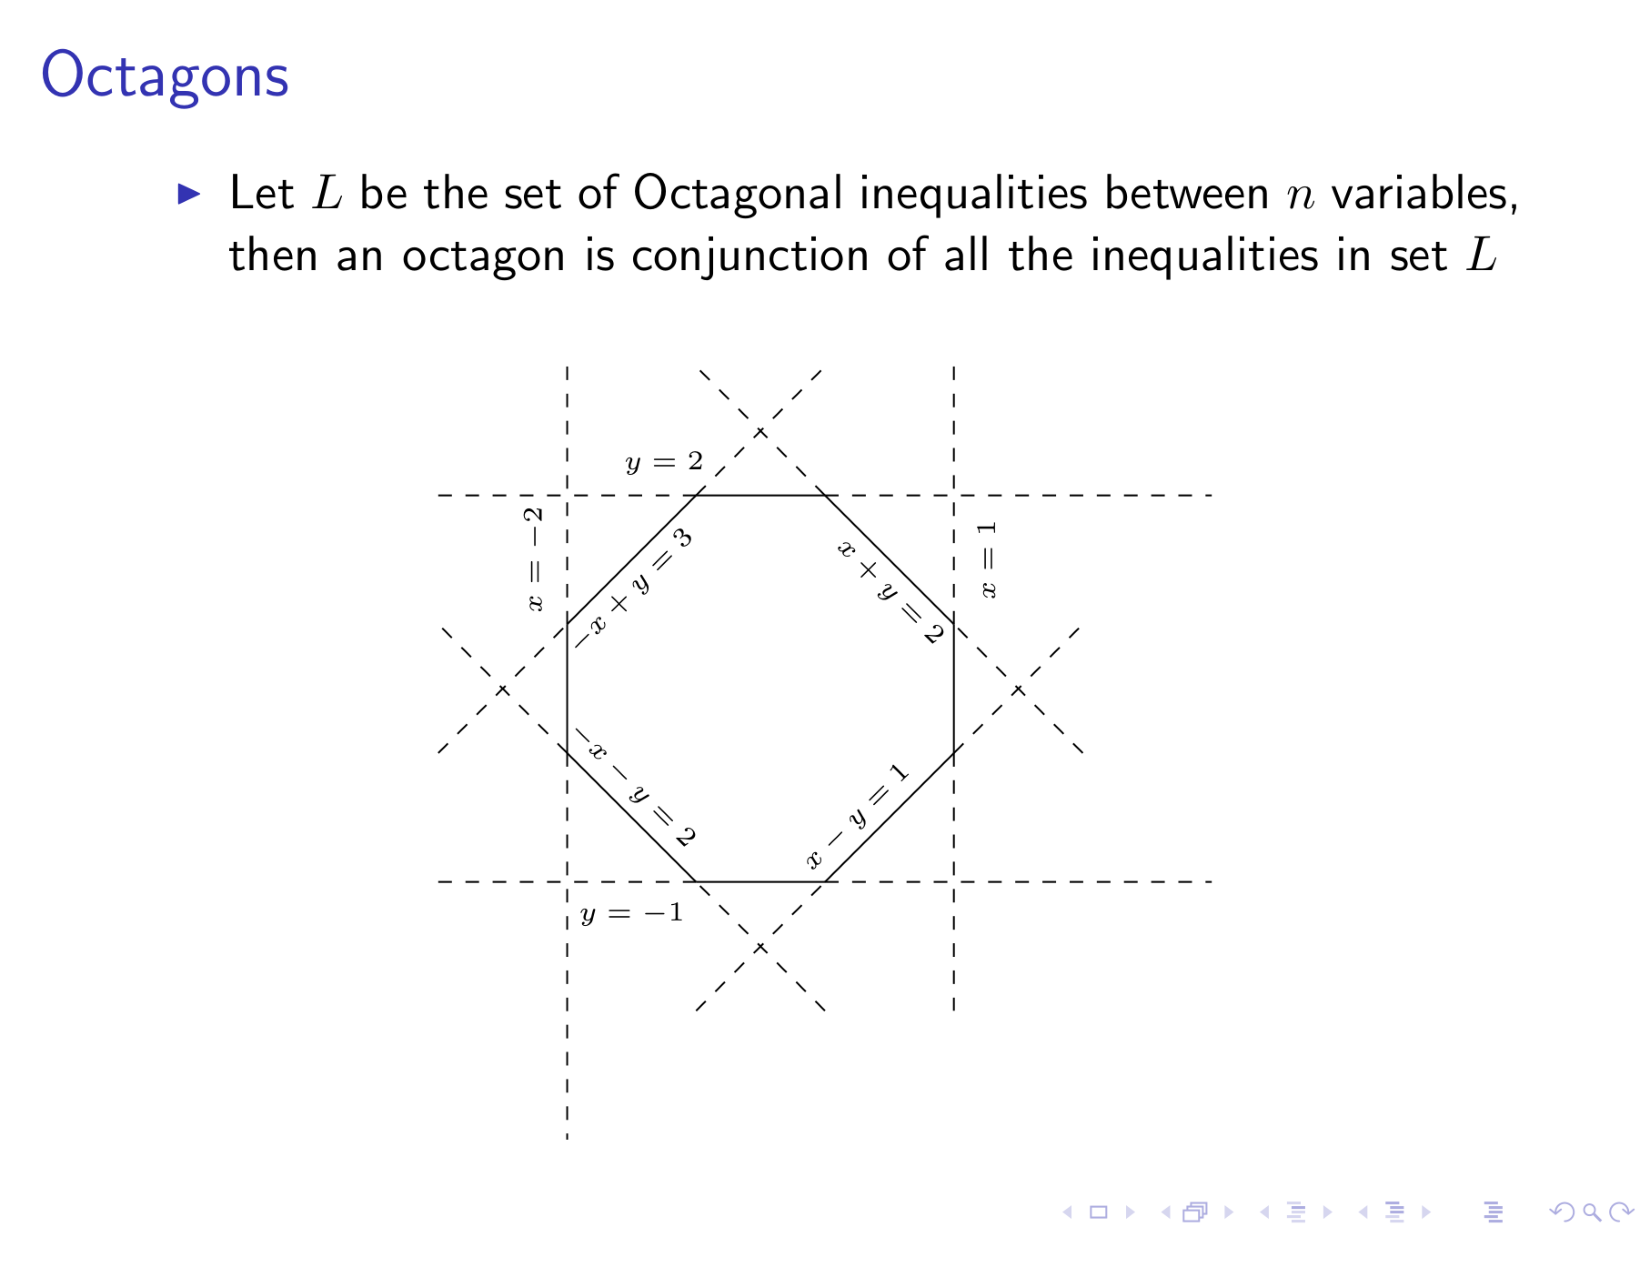
\includepdf[pages={-},nup=1x2, landscape=true]{pages/octagon.pdf}

\section{Encoding}
Matrix $m$ encodes the inequalities. For $k$ Variables $m$ has size $2k \times 2k$. Each $v_i$ is unfolded into $v'_{2i}=v_i^+$ and $v'_{2i+1}=v_i^-$.\\
$m_{i,j}=c$ represents $v'_j -v'_i \leq c$\\
$v_i + v_j \leq c$ can be represented as
\begin{itemize}
\item $v^+_j - v^-_i \leq c$\\
or
\item $v^+_i - v^-_j \leq c$
\end{itemize}
$diag(M)=0$ obviously.
\section{Formalization}
\begin{itemize}
\item The Octagon domain: $(O^O, \sqsubseteq_O, \sqcup_O, \sqcap_O, \bot_O, \top_O)$
\item $\bot_O$ represents bottom element that contains an unsatisfiable set of inequalities.
\item $O$ is the set of all octagons
\item $O^O=O \cup \{\bot_O\}$
\item $T_O$ top element for which the bound for all inequalities is $\infty$
\end{itemize}
\section{Closure(*)}
\label{octagon_closure}
The closure operator produces a unique octagon representation. Binary inequalities such as $v_i - v_j \leq c_1$ and $v_j - v_k \leq c_2$ are comined to obtain $v_i - v_k \leq c_1 + c_2$. If the octagon already contains $v_i - v_k \leq c$ then keep $v_i - v_k \leq min(c, c_1+c_2)$. (This is same as applying Floyd Warshall on the octagon matrix). The set produced by this is maximal and unique.
\section{Least Upper Bound ($\sqcup_O$)}
Union of two octagons is not necessarily an octagon. $\sqcup$ is therefore an approximation. \\
First apply closure to both operands. Then compute union by taking piecewise maximum of bounds of corresponding inequalities. \\
$(x\leq 5) \wedge (x+y \leq 10) \sqcup_O (x\leq 4) \wedge (x+y\leq 11) = (x\leq 5) \wedge (x+y \leq 11)$
\section{Geatest Lower Bound ($\sqcap_O$)}
Intersection of two octagons is always an octagon. Take piecewise minimum of bounds to calculate $\sqcap_O$.
\section{Order ($\sqsubseteq_O$)}
An octagon $O_1$ is included inside another octagon $O_2$ iff the bounds of each inequality in $O_1$ is $\leq$ than the corresponding inequality in $O_2$. Inclusion relation is used for octagon ordering. The closed octagon is the smallest octagon as per $\sqsubseteq_O$ among the set of octagons abstracting the same concrete values.
\section{Widening ($\nabla_O$)}
Widening requires the first operand to not be closed. Widening increases the number of inequalities with $\infty$ whereas closure doeas the reverse. To widen just set the bound to $\infty$ if it increases.
\section{Transformers}
\subsection{Assignment}
Transformer is precise for octagonal assignments but only approximate for those non octagonal.\\
\textbf{Octagonal assignments:}
\begin{itemize}
\item $x=c$ \\
Add inequalities $(x \leq c)$ and $(-x \leq c)$ to the octagon and \underline{close} it.
\item $x = x + c$\\
Subtract $c$ from inequalities having negative coefficient for $x$. Add $c$ to inequalities having positive coefficient for x. The result \underline{is already closed}. 
\item $x = y + c$\\
Add inequalities $(x-y\leq c)$ and $(y-x \leq c)$ to the octagon and \underline{close} it.
\end{itemize}
\textbf{Non-octagonal Assignments:}
$x_j = e$ where $x_j - e$ is non octagonal. 
\begin{enumerate}
\item Compute bounds $[a,b]$ for $e$ using interval arithmetic\\
E.g $e = [a_0, b_0] + \sum_{i=0}^n[a_i,b_i]x_i$ where each $x_i$ has bounds $[c_i,d_i]$ then $[a,b]=[a_0,b_0]+\sum_{i=1}^n[a_i,b_i] \times [c_i,d_i]$
\item Add constraints of the form $\pm x_i \pm x_j \leq [a,b] \pm [c_i,d_i]$ to the octagon.
\item close the octagon
\end{enumerate}
\subsection{Conditional Statements}
Conditional statements encode constraints which can be added to the input octagon. There are octagonal and non octagonal constraints. Similar to assignment octagonal constraints are precise whereas the other constraints are approximated.
\section{Example}
\textbf{See page 24} 
1\chapter{Numerical domains III: Pentagons}
\section{General}
\begin{itemize}
\item Pentagon domain is a reduced product of two domains: Interval ($c \leq x \leq d$) and Strict Upper Bounds (SUB) ($x < y$)
\item Quadratic space complexity
\item Quadratic time complexity
\item Useful for checking array out of bounds error
\begin{itemize}
\item interval component takes care of index underflow ($index \geq 0$)
\item the SUB component takes care of index overflow ($index < array.length$)
\end{itemize}
\end{itemize}
\section{Domain of Strict Upper Bounds (SUB)}
\begin{itemize}
\item for each variable $x$ store the list $s(x)$ of all other variables $y$ s.t. $x<y$
\item SUB domain: $\{S^S, \sqsubseteq_S,\sqcup_S,\sqcap_S,\bot_S,\top_S\}$
\item $\bot_S \iff \exists x,y$ s.t., $y \in s(x) \wedge x \in s(y)$
\item $S$ is the set of all SUB inequalities, $S^S=S \cup \{\bot_S\}$
\item $\top_S \iff \forall x,s(x)=\emptyset$
\end{itemize}
\section{Formalization}
\begin{itemize}
\item $s_1 \subseteq_S s_2 \iff \forall x, s_1(x) \supseteq s_2(x)$
\item $s_1 \sqcup_S s_2 = \forall x.s_1(x) \cap s_2(x)$
\item $s_1 \sqcap_S s_2 = \forall x.s_1(x) \cup s_2(x)$
\item $s_1 \nabla_S s_2 = \forall x.s_1(x) \subseteq s_2(x) ? s_2(x) : \emptyset$
\item Closure is not performed to avoid cubic complexity. 
\begin{itemize}
\item therefore no galois insertion 
\item Domain loses precision for various operators
\end{itemize}
\end{itemize}
\noindent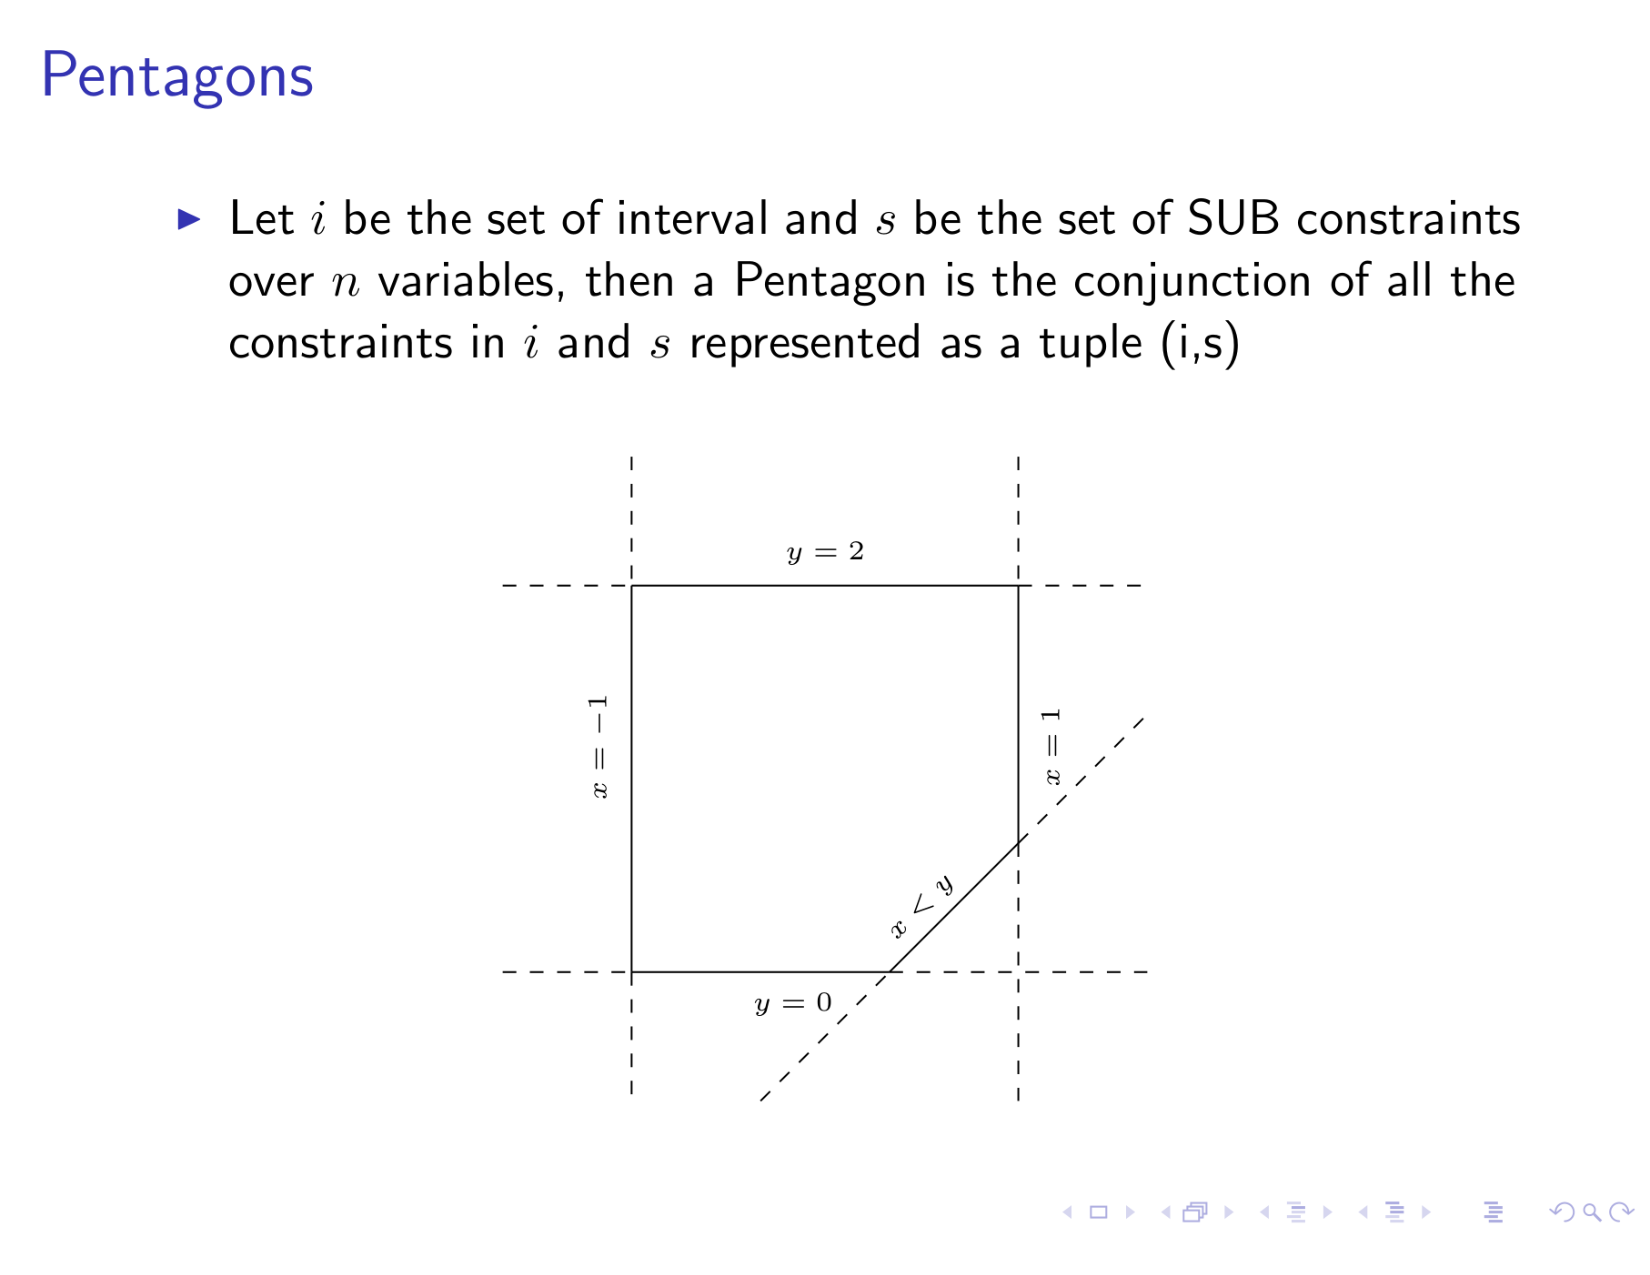
\includepdf[,landscape=true,nup=2x2,pages={-}]{pages/pentagon.pdf}

\chapter{Applications: Analysis of HPC/GPU programs}
\section{Motivation}
Due to FJ, Cilk, X10, DPJ, TPL, CUDA there's renewed interest in structured parallel languages. Determinism is wanted in applications that use such languages. There are lots of parallel algorithmis: Scientific Computing, Signal Processing, Encryption, Sorting, Searching, String Indexing\\
\textbf{Determinism}: for the same input, produce the same output.

\section{Goal}
Prove determinism. Any pair of terminating executions starting with \underline{equivalent input} states, end in \underline{equivalent output} states. Proving arbitrary programs deterministic is hard, instead, we prove a \underline{stronger} property which implies determinism: \textbf{Conflict-Freedom} meaning, parallel threads always access disjoint memory.
\begin{enumerate}
\item Compute all reachable concrete states
\item Check if each state is conflict-free
\end{enumerate}
We denote conflict as a state where 2 threads are \underline{enabled} to access the \underline{same} memory location and one of these accesses is a write.
\textbf{Checking Conflict-Freedom is potentially unbounded.}

\section{Conflict-free Checker}
\label{conflict_free_checker}
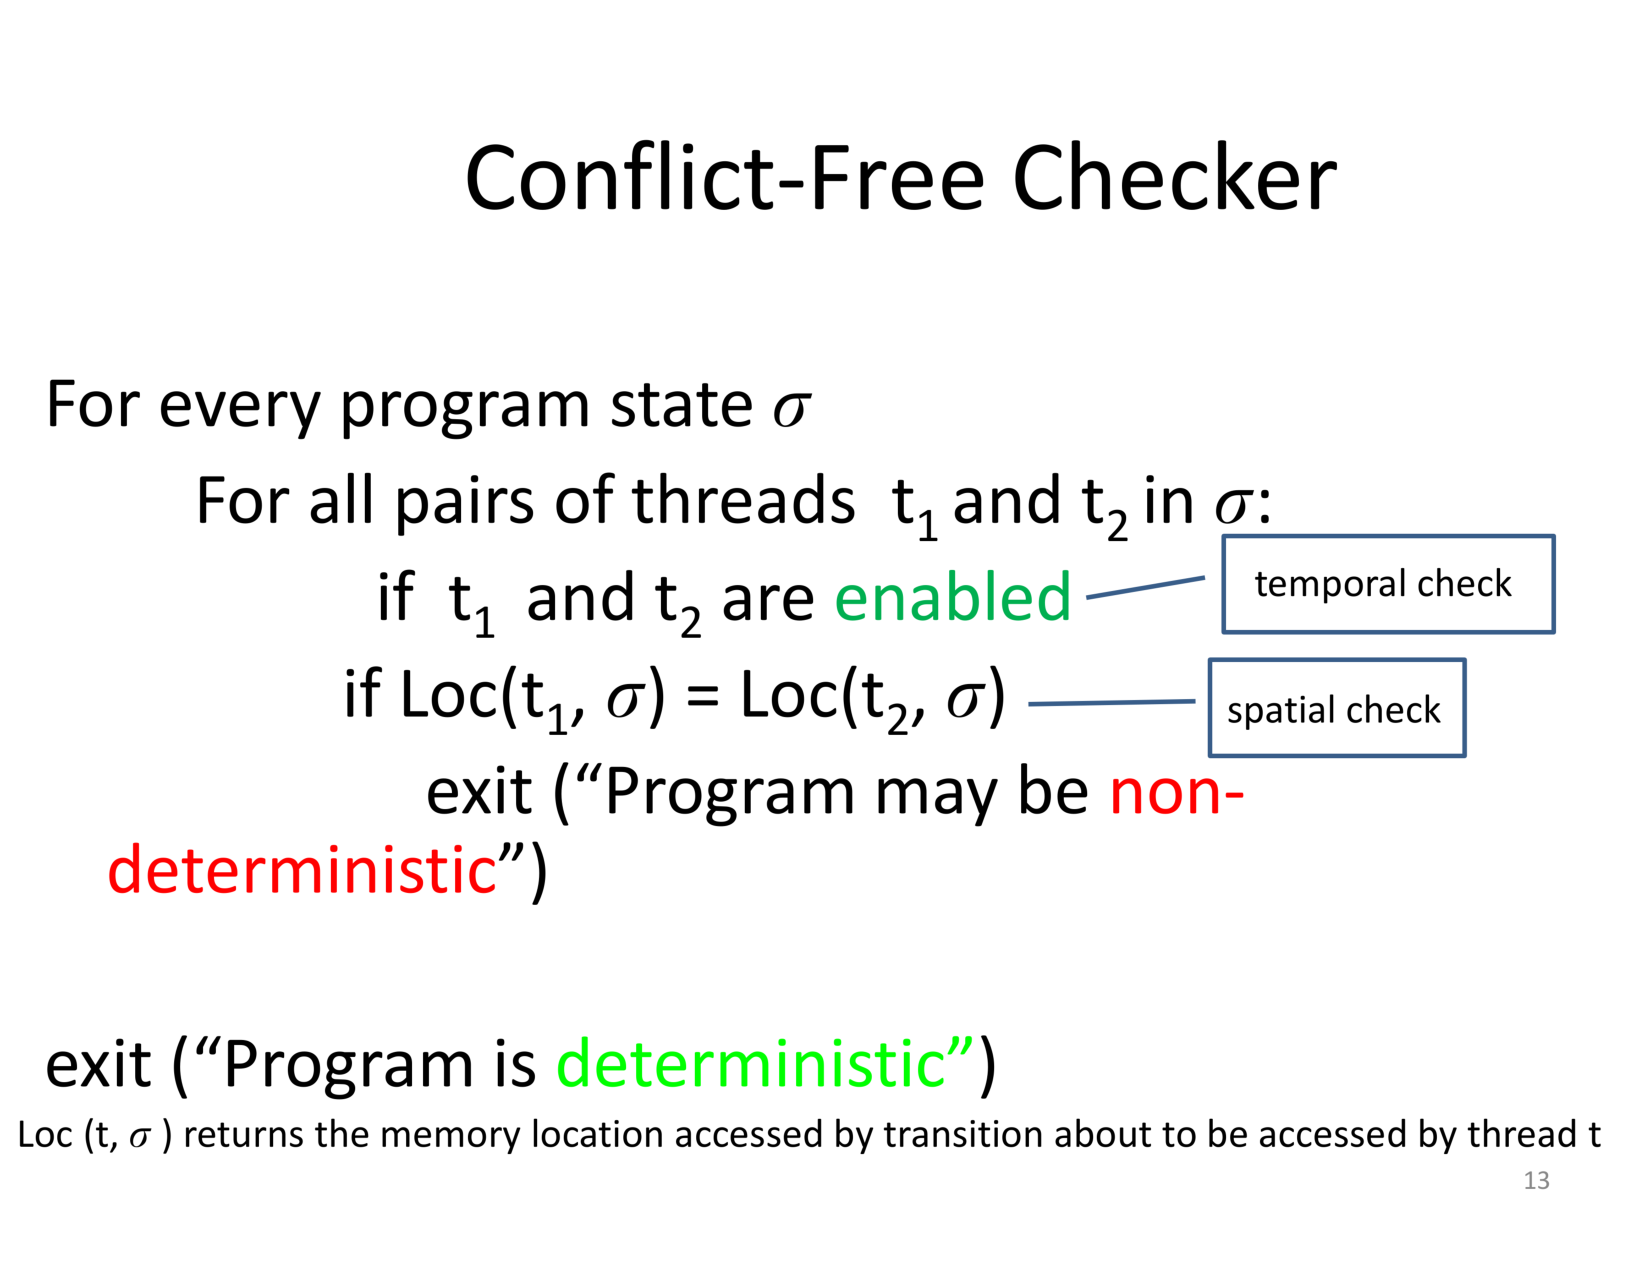
\includepdf[pages={-}]{pages/conflict_free_checker.pdf}

\section{Unboundedness}
Heap, range of array indices and number of threads is unbounded. \\
\textbf{Dealing with Unboundedness}
\begin{itemize}
\item Unbounded Heap
\begin{itemize}
\item Compute finite set of abstract locations
\item Using flow-insensitive \textbf{points-to analysis}
\end{itemize}
\item Unbounded range of array indices
\begin{itemize}
\item Compute symbolic index constraints
\item Using \textbf{numerical abstractions}
\end{itemize}
\item Unbounded number of threads (not discussed in class)
\end{itemize}
\subsection{Points-to Analysis}
\subsubsection{Terms}
Two pointers p and q are \underline{aliases} if they point to the same memory location. $(p,A)$ is a \underline{points-to pair} where $p$ holds the address of object $A$. For two points-to pairs $(p,A),(r,A)$ $p$ and $r$ are aliases.
\subsubsection{Allocation Sites}
Heap is divided into a fixed partitions. All objects \underline{allocated at the same program point} ge represented by a single "abstract object".
\section{Flow-Insensitive Analysis}
Just ignore if conditions and look at every statement for points-to analysis. E.g
\begin{verbatim}
p := new Array 5; // allocation site A1
q := new Array 5; // allocation site A2
if p=q then
	z := p
else
	z := q
\end{verbatim}
will output $points-to(z)={A1, A2}$.

\section{Computing abstract states}
Using \underline{sequential} analysis (based on numerical analysis and pointer analysis) we compute for each thread. \textbf{see Page 34}. First we build for each label (program line) the \underline{abstract states}. E.g. $\sigma_1=\{pc=1,idx=2*tid-ps\}$ for a first program line looking like: \begin{verbatim}
void update(double[][] G, int start, int last, double c1, double c2, int nm, int ps){
   for(tid=start; tid<last; tid+=1){
1:     double [] Gi = G[i];
...
   }
}
\end{verbatim}
For each thread id ($tid$) we can the build \underline{cartesian states}. E.g for $tid=1$ and label 1 ($pc_1=1$):\\
$pc_1=1,ps=0,idx_1=2\\
pc_1=1,ps=1,idx_1=1\\
pc_1=1,ps=2,idx_1=0$\\
And for $tid=4$:\\
$pc_4=1,ps=0,idx_4=8\\
pc_4=1,ps=3,idx_4=5\\
pc_4=1,ps=7,idx_4=1$\\
Combining cartesian states for different threads will give us the \underline{program states}: \\
$pc_1=1,idx_1=2,pc_4=1,idx_4=8,ps=0$ \\
Since $ps$ is a parameter to the function combining two cartesian states with different $ps$ values does not make sense. But it's OK to combine two threads but on different program lines ($pc_i=k,pc_j=k',k\neq k',i\neq j$).\\
\textbf{Summary}:
\begin{itemize}
\item compute invariants for each thread. denote computed values using an expression
\item build cartesian states. "fill" in the missing values to compute variables (many possible combinations).
\item combine abstract states for different threads.
\end{itemize}
Recall the conflict free checker: \ref{conflict_free_checker}. Using the abstract states we can now define an abstract conflict-free checker:
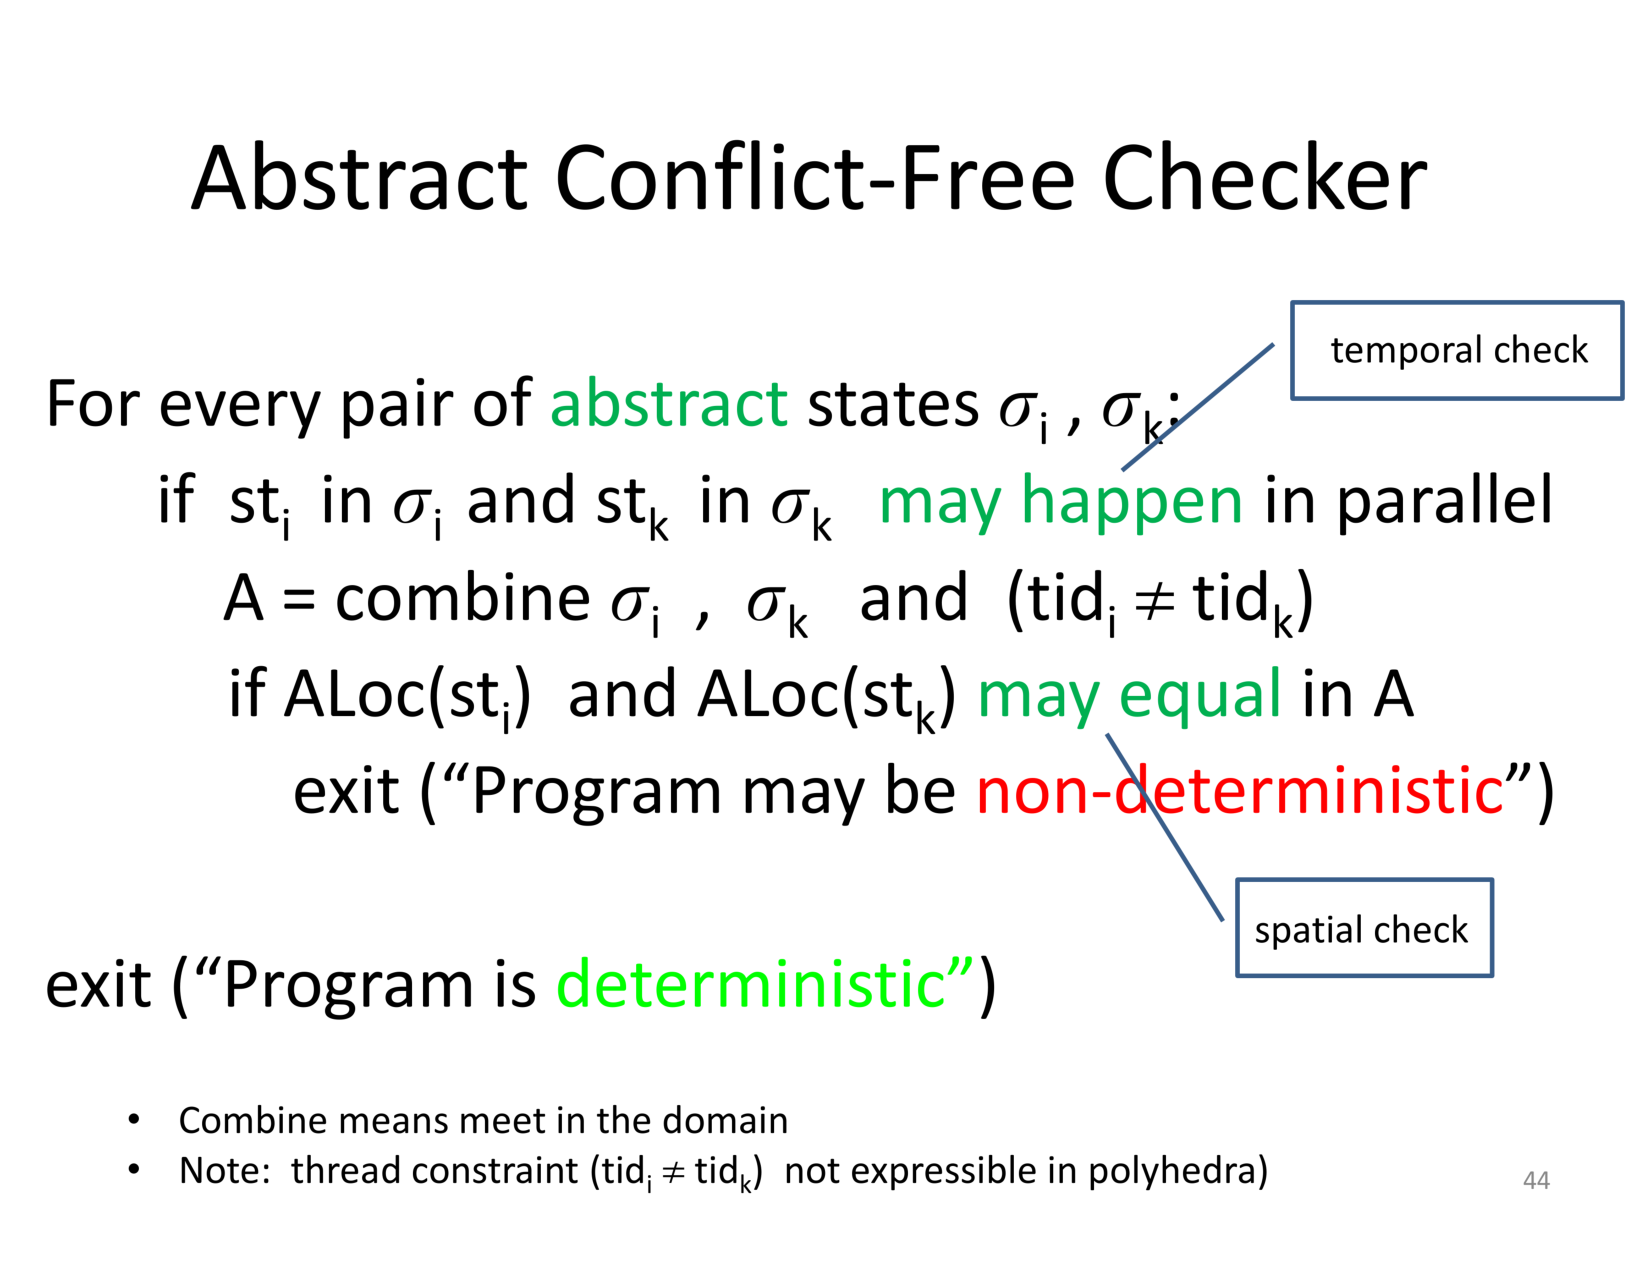
\includepdf[pages={-}]{pages/abstract_conflict_free_checker.pdf}
A \underline{may happen} analysis can be used for the may happen parts. There are many works on this. \textbf{TODO}?
\section{May Equal (Arrays) / Abstract Locations}
$ALoc(G[i]=128) := (G,i)$ with $G$ a pointer- and $i$ and integer variable. When may two $ALoc(a,i)$ and $ALoc(b,k)$ equal? When $(a $ may alias $ b) \wedge (i $ may overlap $ k)$. With may alias=$points-to(a) \cap points-to(b) \neq \emptyset$ and may overlap=$A_N \sqcap (i=k)\neq \bot$ \textbf{TODO: not sure what $A_n$ is. page 49}
\section{Caveats}
Heap abstraction is imprecise. 
\begin{itemize}
\item Aliasing information \underline{inside} reference arrays is lost. Example: \begin{verbatim}
Object A[], double G[][];
\end{verbatim}
\item So, points-to information is not enough
\item We want $\forall i,j,A:i \neq j \implies A[i] \neq A[j]$ but this is very difficult to prove in general.
\end{itemize}
\subsection{Domain-specific solution}
Most numerical HPC/GPU programs initialize reference arrays only with fresh objects \textit{A[i] = new Object();} and never update afterwards. Easy to prove as a global invariant.
\section{Implementation}
\begin{itemize}
\item Soot (Analysis works on Jimple intermediate representation)
\item Apron library (for numerical invariants)
\item Benchmarked using Java JGF benchmarks
\end{itemize}

\section{Limitations}
\begin{itemize}
\item cannot handle some kinds of non-linear constraints (\textit{A[x*N + z]=c} where N never changes
\item atomic sections
\item Accesses from nested primitive arrays: \textit{A[ B[i] ] = 5} where \textit{B[i]}'s are distinct
\end{itemize}
\section{Recap}
To automatically prove determinism prove a \underline{stronger property}: conflict-freedom. % Applications: Analysis of HPC/GPU programs
\chapter{Applications: Semantic Program Differencing}
\section{Motivation}
Do two programs behave the same. Has an example \textit{print\_numbers\_v\_6\_9()} and \textit{print\_numbers\_v\_6\_10()} with syntactic differences but the same output. Are they the same? When running the programs and comparing the difference you can only spot cases where procedures differ. You cannot prove equivalence for most programs. \textbf{Abstract Semantic Differencing} FTW! Either prove equivalence or \underline{characterize their difference} (find differing program states that come from the same input).\\
\underline{Sound}: Equivalence guaranteed
\underline{Precise}: Report few differences
\subsection{Equivalence under abstraction}
Equivalence under abstraction does not entail equivalence between the concrete values it represents.
\section{Their Approach}
Nimrod Partush, Eran Yahav, Technion, Israel\\
\begin{itemize}
\item Analyze P and P' together
\begin{itemize}
\item define \underline{correlating semantics} that interprets the programs together
\item Interpret in some ordering of their steps
\item Abstract the correlating semantics (to handle infinite-state programs)
\end{itemize}
\item Search for the program ordering that allows the abstraction to \underline{best capture equivalence}.
\end{itemize}
Idea: join ($\sqcup$) states only if they hold equivalence for the same variables. \\
$\{x<0,res=res'=-1\} \sqcup \{x>0,res=res'\} = \{x = \top, res=res' = [-1,1]\}$
\subsection{Finding the Analysis Order}
Sequential order has problems: When one programs analysis has finished its values have been abstracted and equivalence is lost. 
Imagine a $M=n \times m$ Matrix here. $m_{1,1}$ is the abstract state where both programs are on line 1. How do we check the states?\\
\begin{itemize}
\item sequential $m_{1-n,1}$ then $m_{n,1-m}$:\\ 
fails to see that two identical programs are equivalent (they never interesect on a state).
\item Lock-step $m_{1,1}, m_{2,1}, m_{2,2}, m_{3,2}$:\\
fails for programs with different number of lines
\item all possible interleavings:\\
need ot check \underline{every} element of $M$ (aka every possible interleaving)
\end{itemize} 
\subsection{Correlating Programs}
\subsubsection{Previous work (SAS 13')}
Previously they joined the programs into one program which holds both program semantics. Assumed syntactic similarity and used a syntactic diff. Transformation tool \textit{ccc} is available on github. \\
\textbf{Problem}: when syntactc difference is vast, the composition will be sequential. Leads to imprecise (and useless) results. 
\subsubsection{Speculative Exploration}
Using a \underline{speculation window} $k$ both programs are epxplored $k$ steps distributed over both programs. 
\begin{itemize}
\item 0 over P and $k$ over P'
\item 1 over P and $k-1$ over P'
\item etc.
\end{itemize}
\textbf{TODO: read again.} % Abstract Semantic differencing via speculative correlation
\chapter{SMT theories \& Symbolic Execution}
\section{Intro}
Validity in first order logic (FOL) is undecidable, while validity in particular first order theories is (sometimes) decidable. These theories allow us to capture structures which are used by programs (arrays, ints etc.) and enable reasoning about them. \\
Formulas in each theory are constructed with a specific set of function, predicate and constant symbols. This is the \underline{signature} of the theory called $\Sigma$. Using $\Sigma$, logical connectives ($\wedge, \to$) and quantifiers first order formulas can be built. Each theory comes with a set of \underline{axioms} (FOL formulas) called $A$, which only contain elements form the signature. A formula F in the theory \underline{is valid} if all interpretations that satisfy the axioms in $A$ also satisfy the formula. Some theories are meant to be used with a \underline{particular interpretation} (e.g. in theory of integers formulas are interpreted over ints). A \underline{fragment} of a theory consists of a subset of the possible formulas expressible in the theory. A theory is \underline{decidable} if for every formula in the theory we can automatically check whether the formula is valid or not. Similarly for fragments of a theory.
\section{Decidability}
Decidability is mainly needed to achive 100\% \underline{automation}. If the theory is not decidable sometimes the theorem prover (e.g. Z3, Yices) which is used may succeed.
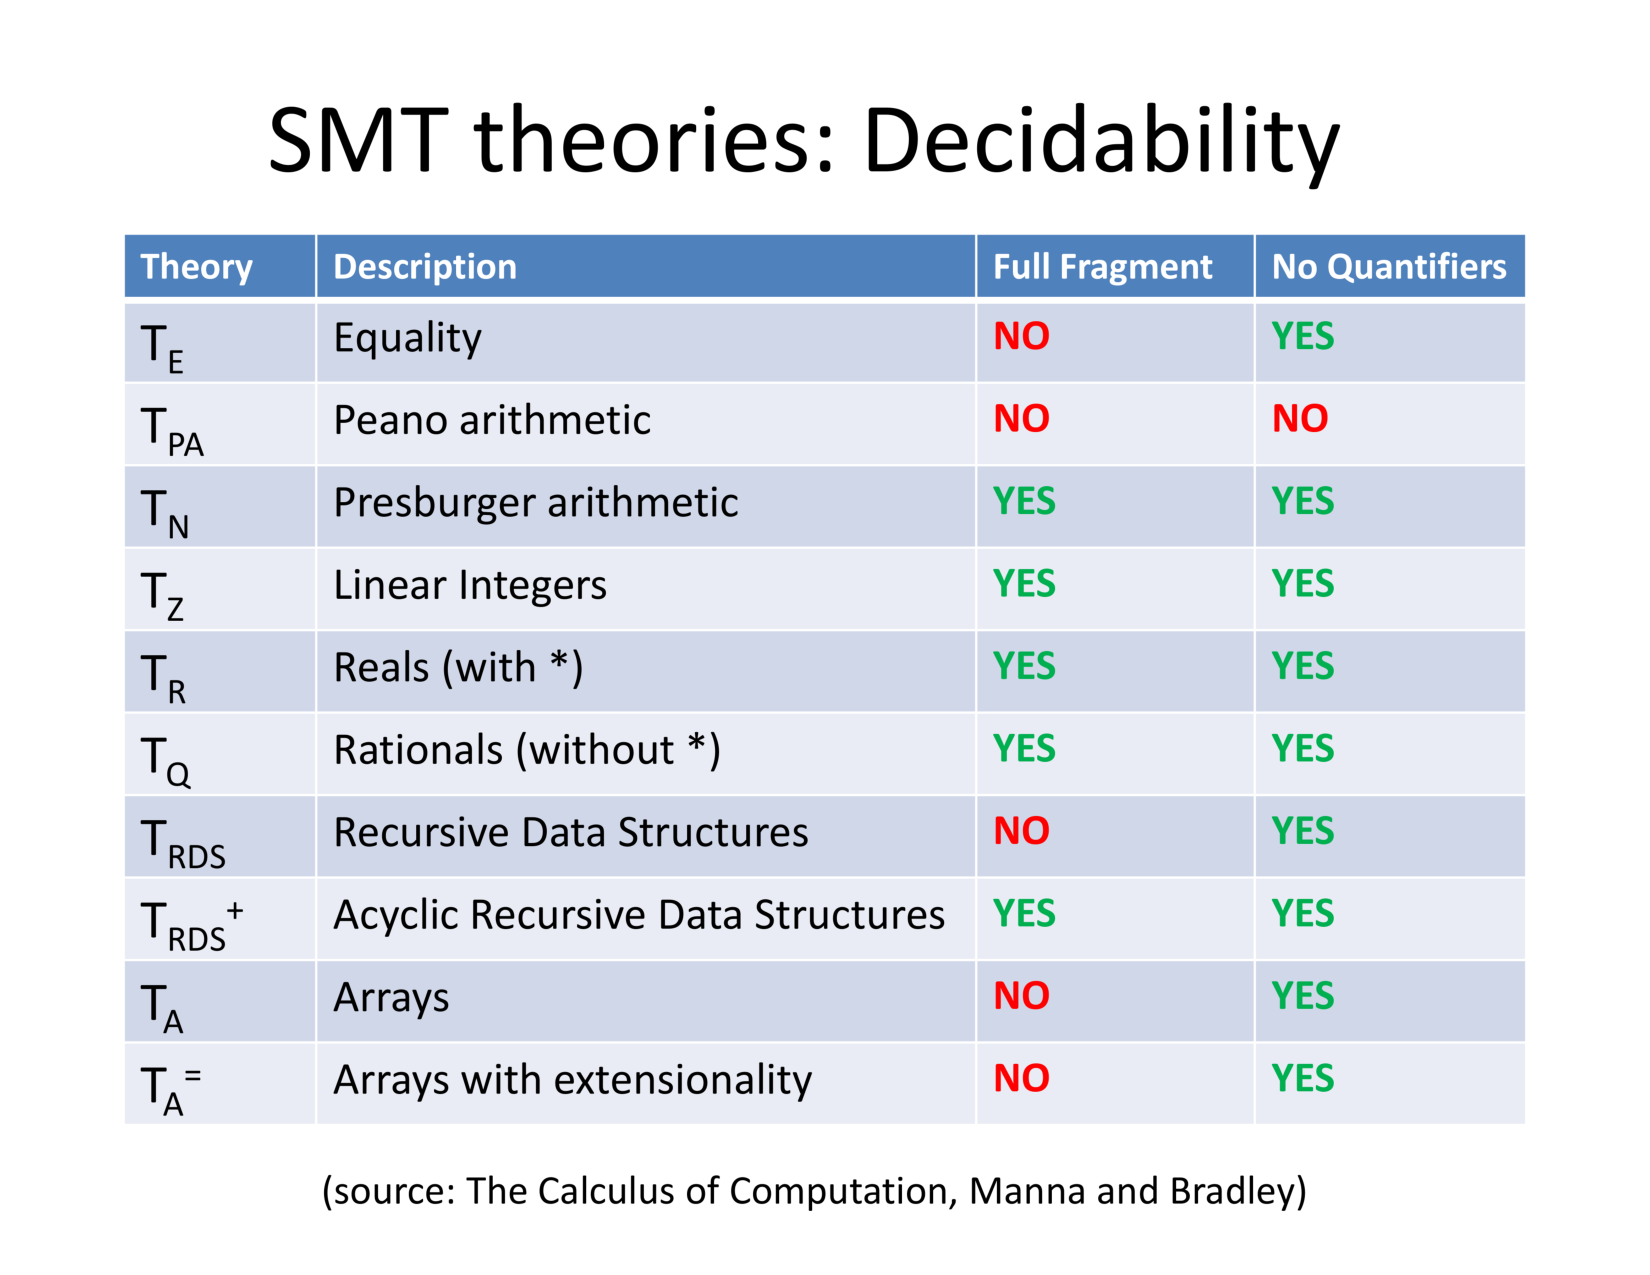
\includepdf[pages={-}]{pages/decidability.pdf}
\section{TODO}
pages <24 with all those theories.
\section{Symbolic Execution}
Widely used in practice. Symbolic Execution keeps two formulas at any point during program execution: \textbf{symbolic store} and a \textbf{path constraint}. The \underline{symbolic state} is the \underline{conjuction} of these two formulas.
\subsection{Existing Tools}
Stanford's KLEE, NASA's Java PathFinder, Microsoft Research's SAFE, UC Berkeley's CUTE, EPFL's S2E.
\subsection{Symbolic store}
$\sigma_s:Var \to Sym$ maps each variable to a value at any given time. Example: $\sigma_s: x \mapsto x0, y \mapsto y0$
\subsection{Semantics}
Arithmetic expression evlauation simply manipulates the symbolic values. Let $\sigma_s: x \mapsto x0, y \mapsto y0$ Then, $z=x+y$ will produce the symbolic store: $x \mapsto x0, y \mapsto y0, z\mapsto x0+y0$ 
\subsection{Path Constraint}
Records all branches taken so far. Typically a decidable logical fragment without quantifiers. Is \underline{true} at the start of the analysis. Evaluation of \underline{conditionals} affects the path constraint but not the symbolic store.
\subsection{Limitation: Loops}
Unbounded loops run forever in symbolic execution. Easiest soluton: provide some loop bound meanging \underline{under-approximate}(under-approximation: only feasible paths?\textbf{TODO}). Another solution is to provide \underline{loop invariants}. But this is rarely used for large programs because it's difficult to provide such invariants manually and it can lead to \underline{over-approximation}. \underline{Static analysis can infer loop variants.} 
\subsection{Constraint solving}
It's important that
\begin{enumerate}
\item  a SMT solver suppoerts as many decidable logical fragments as possible (some tools even use more than one SMT solver)
\item  a SMT solver can solve large formulas quickly
\item the symbolic execution engine tries to reduce the burden in calling the SMT solver by exploring domain specific insights.
\end{enumerate}
A key-optimization is obviously \underline{caching}. The symbolic execution engine can keep a map (cache) of formulas to a satisfying assignment for the formula. For new formulas it can the first access the cache before calling the SMT solver.
\subsection{Concolic Execution - When constraint solving fails}
SMT solvers do not handle \underline{non-linear constraints} well (e.g z = y*y, ... page 47).
Concolic Execution combines \underline{both} symbolic execution and concrete (normal) execution. The program runs as usual (with some input that needs to be given) and also maintains the symbolic information. For example when there's a \textit{read()} use two stores. one with actual values (e.g. 22,1, etc.) and one with the symbolic information. Run several times. If for example the then branch is reached and we need the else brnach. negate path constraint and run againe. See examples on page 49. % SMT theories & Symbolic Execution
\chapter{Predicate Abstraction and Concurrency}
\section{Introduction}
Predicate Abstraction is used to automatically verify: C device drivers (SLAM project at MSR), distributes concurrent algorithms, biological systems (PRISM at Oxford), security properties.
\section{Theory}
\subsection{Domain}
\subsubsection{Concreate Domain}
$Lab \to p(Store)$ \textbf{TODO: powerset symbol?}\\
e.g. $2 \to \{\{x=1,y=3\},\{x=2,y=2\}\}$
\subsubsection{Logical Domain}
Capture the set of stores with a FOL formula. Example:\\
$1 \to x=1 \wedge y=2\\
2 \to (x=1\wedge y=3) \vee (x=2\wedge y=2)$
Then a Galois Connection between $Lab \to p(Store)$ and $Lab \to FOL$ can be setup.
\subsection{Concrete Transformers}
$F^{FOL}:(Lab \to FOL) \to (Lab \to FOL)$\\
$F^{FOL}(m)l = \begin{cases} true &\mbox{if l is initial label}\\ 
\bigvee_{(l',action,l)}\llbracket action \rrbracket_{FOL}(m(l')) & \mbox{otherwise}\end{cases}$
\subsubsection{Effect of action on a FOL formula}
$\llbracket action \rrbracket_{FOL}: FOL \to FOL$\\Examples: \\
$\llbracket skip \rrbracket_{FOL}(x=1 \wedge y=2) = (x=1 \wedge y=2)\\ \llbracket (x > 5)\rrbracket_{FOL}(x>0 \wedge y=2)=(x>5 \wedge y=2)\\ \llbracket (x:=7) \rrbracket_{FOL}((x<0) \wedge (x=5)) = (x=7)$
\subsubsection{Strongest post condition}
The \underline{best transformer} for $\llbracket action \rrbracket_{FOL}$ is the strongest post-condition (sp).\\
$\llbracket action \rrbracket_{FOL}(\psi) = sp(\psi, action)$\\
With $sp(\psi, action) = \psi'$ The formula $\psi'$ si the most precise (strongest) set of successor stores of $\psi$ as determined by action.\\
$sp(\psi, skip) = \psi\\
sp(\psi, b) = \psi \wedge b\\
sp(\psi, x:=a) = \exists v:x=a[v/x] \wedge \psi[v/x]$\\
Quantifiers are difficult to handle for automated reasoning engines and many decidable fragments do not allow quantifiers.
\subsubsection{Weakest Pre-Condition}
$wp(\psi, skip) = \psi\\ wp(\psi,b) = b \Rightarrow \psi\\ wp(\psi, x:=a) = \psi[a/x]$\\
\textbf{No quantifiers!}
\subsubsection{linking sp with wp}
\begin{theorem}
$sp(\psi, action) \Rightarrow \psi' \equiv \psi \Rightarrow wp(\psi', action)$
\end{theorem}
Using weakest preconditions we get rid of quantifier. \textbf{TODO}: check again. 
\subsubsection{Undecidability}
FOL is undecidable. If $\psi$ in FOL is not valid, the no algorithm is guaranteed to terminate. Can't guarantee termination of iterating $F^{FOL}$.
\section{Predicate Abstraction recipe}
\begin{enumerate}
\item Come up with an \underline{abstract domain} (based on the type of properties you want to prove)
\item Define abstract semantics \underline{for the programming language} w.r.t. the abstract domain from step 1.
\begin{itemize}
\item define the abstract transformers (effect of statement on the domain)
\item prove that the abstract semantics are \underline{sound} w.r.t \underline{concrete semantics} of the programming language
\end{itemize}
\item iterate abstract transformers over the abstract domain until fixed point
\end{enumerate}
\subsection{Abstract domain}
We define $F$ to be a \underline{finite} set of predicates $F=\{\phi_1, \phi_2,... \phi_n\}$ where the predicates are selected from a \underline{decidable} logical fragment. Examples for the predicates are: \\$\phi_1 := x > 0 \wedge x = (x+1)\\ \phi_2:=z+y>5 \wedge x=(y+y)$ (over theory of integers).\\
Using the predicates we define a \underline{cube} which is a \underline{conjuction} of predicates and negated predicates where each $\phi_i$ appears \underline{at most once}. Cubes can be represented as vectors of size n where the value at index $i$ indicates if $\phi_i$ is negated (0), positive (1) or missing (T).\\ \\
Our resulting abstract domain is $Lab \to Cube_F$ where $Cube_F$ is the set of all possible cubes formed over the predicates in $F$.\\ \\ 
Let's define $\sqsubseteq_{pa}, \sqcap_{pa}, \sqcup_{pa}$:
\begin{itemize}
    \item Ordering $\sqsubseteq_{pa}$: 
        \begin{itemize}
            \item $a \sqsubseteq_{pa} b$ compares the elements pointwise
            \item $a \sqsubseteq_{pa} b $ means $a \Rightarrow b$, but not vice versa
            \item Examples:\\
                $101 \sqsubseteq_{pa} 100 = no\\ 100 \sqsubseteq_{pa} 101 = no\\T01 \sqsubseteq_{pa} 10T = no\\011 \sqsubseteq_{pa} 01T = yes\\01T \sqsubseteq_{pa} 011 = no$
        \end{itemize}
    \item Greates lower bound $\sqcap_{pa}$
        \begin{itemize}
            \item keep $\phi_k$ unsell $\phi_k$ appears in a, and $\neg \phi_k$ appears in b (or vice versa) in which case $a \sqcap_{pa} b$ returns false
            \item Examples: $101 \sqcap_{pa} 100 = false\\101 \sqcap_{pa} 10T = 101\\ T01 \sqcap_{pa} 10T = 101\\ 00T \sqcap_{pa} 01T = false$
        \end{itemize}
    \item Least upper bound $\sqcup_{pa}$
        \begin{itemize}
            \item predicate (or negation) is kept if it appears in both cubes. 
            \item if all predicates are ommited then $\sqcup_{pa}$ returns true
            \item $a \vee b \Rightarrow a \sqcup_{pa} b$
            \item Examples:\\ $101 \sqcup_{pa} 100 = 10T\\101 \sqcup_{pa} 010 = true\\T01 \sqcup_{pa} 10T = T0T\\true \sqcup_{pa} 011 = true$
        \end{itemize}
\end{itemize}
\subsubsection{Connection Domains - Galois Connections}
Next we setup a Galois connection between FOL and $Cube_F$
Concretization: $\gamma: Cube_F \to FOL\\ \gamma(cube) = cube$\\ $\alpha$ is defined by $\gamma$ and vice versa. So: \\
$\alpha(\psi) = \sqcap_{pa}\{cube | \psi \sqsubseteq_{FOL}\gamma(cube)\}$ \textbf{TODO:} where is this definition from?\\
In FOL, $\sqsubseteq_{FOL}$ is: $\alpha(\psi) = \sqcap_{pa}\{cube | \psi \Rightarrow \gamma(cube)\}$ By substitution of $\gamma$ we get:\\
\underline{$a(\psi)=\sqcap_{pa}\{cube|\psi \Rightarrow cube\}$}\\
Example:\\
$F=\{(2x-y), (y*y>4), (x+y<5)\}\\
\alpha(x=1 \wedge y=3) = \sqcap_{pa}\{0TT, T1T, TT1, 01T, 0T1, T11, 011\} = 011 = \neg(2x-y>0)\wedge (y*y>4)\wedge x+y<5$\\
\textbf{Optimization}: instead of $\alpha(\psi)=\sqcap_{pa}\{cube | \psi \Rightarrow cube\}$ use $\alpha(\psi)=\sqcap_{pa}\{literal|\psi \Rightarrow literal\}$
$literal \iff cube$ has only one value different that T in the correpsonding array. Example: 0TT, T1T. \textbf{TODO: no idea here, page 28}\\
\textbf{TODO: why is this a galois connection?}
\subsection{Abstract Transformers}
\textbf{TODO: pretty cool construction of abstract transformer}\\
$\llbracket action \rrbracket_{FOL}(\psi) = sp(\psi, action)$ is the best concrete transformer. \textbf{Why?} Now lets defined the \underline{best abstract transformer}: $\llbracket action \rrbracket_{pa}:Cube_F \to Cube_F$
\begin{align}
    \llbracket action \rrbracket_{pa}(c) 
    &= \alpha \circ \llbracket action \rrbracket_{FOL} \circ \gamma(c)
    \\&= \alpha \circ \llbracket action \rrbracket_{FOL}(c) && \text{substitution of $\gamma$}
    \\&= \sqcap_{pa}\{literal | \llbracket action \rrbracket_{FOL}(c) \Rightarrow literal\} && \text{definition of $\alpha$}
    \\&=\sqcap_{pa}\{literal | sp(c,action) \Rightarrow literal\} &&\text{definition of $\llbracket action \rrbracket_{pa}$}
    \\&=\sqcap_{pa}\{literal | c \Rightarrow wp(literal, action)\} &&\text{by sp to wp connection}
\end{align}
So to compute the tranformer, we need to check whether the formula $c \Rightarrow wp(literal, action)$ is \underline{valid}. This is done with an SMT solver and it's therefore desirable that the formulas are in some decidable logical fragment.
\subsubsection{Key points}
\begin{itemize}
    \item for predicate abstraction the transformers are proved correct once and for all
    \item then we can instantiate predicate abstraction with any predicates and don't need to prove correctness
    \item in that sense predicate abstraction is a parametric framework
    \item the challenge is to find the sufficient predicates
\end{itemize}
\subsection{Iterate to a fixed point}
see page 33.
\subsection{Summary}
\begin{itemize}
    \item we used wp for the best transformer because it introduces no quantifiers
    \item Best abstract transformer is sound by construction
    \item an important challenge is to find the sufficient predicates F to verify the program
\end{itemize}
\subsubsection{An alternative to fidex-point iteration}
\textbf{TODO}: important / good idea?\\ 
Input: a program $P$, a set of predicates $F$ and a property $S$ to verify. 
\begin{enumerate}
    \item Build a boolean program $B(P,F)$\\
        Program contains only boolean variables, one for each predicate in F.
    \item Check that $B(P,F)$ verifies the property $S$. \\
        If the property holds for $B(P,F)$ then it also holds for P.
\end{enumerate}
\textbf{TODO: pages 36-37}
\section{Predicate Abstraction for Modern Concurrency}
\textbf{TODO: } check again. especially the "boolean program" part. 
cube is $O(3^{length})$ used extrapolition to work on cubes $\ll cube$ 

\chapter{Synthesis from Examples}
The goal of synthesis is to learn a program from examples. The key challenge is \underline{generalization}, where we want to generalize from examples to something that is applicable in new situations. How do we generalize from a small number of examples? When do we know we're done? 
\section{Problem Dimensions}
\begin{itemize}
\item Programming languages \\
Need a language expressive enough to capture programs of interest and is amenable to learning.
\item Machine Learning \\
Need to learn a function in the language
\item HCI \\
Input-output based interatictino model
\end{itemize}
\section{Version Spaces}
First some keywords:
\begin{itemize}
\item \underline{hypothesis h}: is a function $h: Input \to Output$
\item \underline{hypothesis space H}: is a set of hypotheses
\item a hypothesis $h$ is \underline{consistent} with a sequence of input-output examples iff $\forall (x,y) \in D: h(x) = y$
\item \underline{version space} $VS_{H,D}$ consists of only those hypotheses in $H$ that are \underline{consistent} with all examples in $D$. $VS_{H,D} \subseteq H$
\end{itemize} 
Version spaces are usually associated with some form of partial order on the hypotheses in $VS_{H,D}$. $h_1 \sqsubseteq h_2 \iff \text{h2 covers more examples than } h_1$ \\ Version spaces can be represented using just 
\begin{itemize}
\item the most general constistent hypothesis (least upper bound)
\item the most specific consistent hypothesis (greatest lower bound)
\end{itemize}
\section{Version Space Algebra}
Let's define \underline{operations} on a version space $VS_{H,D}$
\begin{itemize}
\item combining version spaces
\item joining version spaces
\item transforming version spaces
\end{itemize}
This allows us to build complex version spaces out of simpler ones. Trasnformations are needed because given more examples we'll need to update the version space. 
\subsection{Union}
$VS_{H1,D} \cup VS_{H2,D} = VS_{H1 \cup H2, D}$
For the same set of examples D. The functions in $H1$ and $H2$ have the same domains and ranges.
\subsection{Join}
Used symbol for join: $\bowtie$\\
$VS_{H1,D1} \bowtie VS_{H2,D2} = \{\langle h_1,h_2 \rangle | h_1 \in VS_{H1,D1}, h_2 \in VS_{H2,D2}, C(\langle h_1, h_2\rangle, D)\}$
Where $D1,D2$ are sequences of n inpute-output examples over $H1$ or $H2$ respectively.\\
D is a sequence $\langle (i_1,o_1), (k_1,l_1) \rangle ... \langle (i_n, o_n), (k_n, l_n) \rangle$\\
$C(h,D)$ is a \underline{consistency predicate}, true when hypothesis h consistent in D.
\subsection{Independent join}
Same definition but condition for independence:\\
$\forall h_1 \in H1, h_2 \in H2 . C(h_1, D1) \wedge C(h_2, D2) \implies (\langle h_1, h_2 \rangle, D)$ That's essentially a cartesian product.\\ 
\textbf{Effiency of independent join $\bowtie$}:\\
$Space(VS_{H1,D1} \bowtie VS_{H2,D2}) = Space(VS_{H1,D1}) + Space(VS_{H2,D2})+C1\\ \forall d_1, d_2 . Time(VS_{H1,D1} \bowtie VS_{H2,D2}, \langle d_1, d_2 \rangle) = Time(VS_{H1,D1}, d_1) + Time(VS_{H2,D2}, d2) + C2$
\subsection{Transforms}
Transform one version space into another. Version space $VS1$ is a transform of version space $VS2$ iff: $\text{Let VS1} = \{g | \exists f \in VS2 . \forall i . g(i) = rm^{-1}(f(dm(i)))\}$. Where $dm$ is a map from elements in the domain of functions in $VS1$ to elements in the domain of the functions in $VS2$ and $rm$ is a 1-1 map from elements in the range of functions in $VS1$ to elements in the range of the functions in VS2.
\section{Learning Version spaces}
PAC learnability - probably approximately correct learning - helps us to answer the question "How many examples do we need to learn the target function?".\\
We \underline{run} a version space on an input by applying every function in VS on that input and collecting the outputs. Two hypotheses $h_1,h_2$ may "agree" on some input.
\begin{itemize}
    \item Assign a probability to each hypothesis in the version space
    \item Choosing a probablity allows us \begin{itemize}
            \item to find better hypotheses (those with higher probability)
            \item to specify priors 
            \item to deal with noisy data (by assignin a low probability > 0 to inconsistent hypotheses)
        \end{itemize}
    \item $Pr(h | H)$ denothes the probability associated with hypothesis h in a hypothesis space H
    \item $Pr(Vi | W) $ denotes the prob. of a version space Vi given the version space W which is union of other version spaces
    \item if no prior knowledge, these are the uniform distributions
    \item The prob. of a hypothesis h in a version space V, denoted by $Pr(h | V)$ is updated as the version space changes and inconsistent hypotheses are removed.
\end{itemize}
\subsection{Inductive Definitions of Probabilities}
\begin{itemize}
    \item initially: $Pr(h | V) = Pr(h | H)$
    \item \textbf{Transform}: if version space V1 is a transform of another version space V2, then $Pr(h | V1) = Pr(f, V2)$ with $f$ beging the "matching function"
    \item \textbf{Union}: $P(h | V) = wi * P(h | Vi)$ \\
        V is the union of VI's \\
        wi is the probability of version space Vi\\
        \textbf{TODO, page 20}: werden die aufsummiert oder was? 
    \item \textbf{Join}: $P(h | V)$ is the joint probability of the hypotheses hi, ... hn.\\
        if independent then: $P(h | V) = P(hi | Vi) * ... P(hn | Vn)$
\end{itemize}
Having all those probabilities allows us to sum up all hypotheses that give the same result for a given input.
\begin{equation}
    \label{output_probabilities}
    Pr_v^O(i) = \sum_{\forall h | h(i) = o} Pr(h | V)
\end{equation}
This way we can present to the user the output states with the highest probability.
\section{Example: SMARTedit}
SMARTedit (by Tessa Lau) is one of the first working approaches and for learning interesting programs. It introduces version space algebras (VSA) for learning programs.
SMARTedit is a texteditor that represents it editor state as $\sigma=\langle T,L,P,E \rangle$ with $T$ beging the contents of the text buffer, $L$ the cursor location (row, column), $P$ the contents of the clipboard and $E$ a contiguous region of T representing selected text.\\
\subsection{Action}
An editor \underline{action} is a function $a: \Sigma \to \Sigma$ with $\Sigma$ beging the set of possible editor states.\\
\textbf{Example:}\\
$\langle T, (42,0), P, E\rangle \to \langle T, (43,0), P, E\rangle$
"move to the next line" or "move to the beginning of line 43" are \underline{consistent}. \\
"move to the beginning of line 47" and "move to the end of line 41" are inconsistent.
Actions have locations. E.g move to location, delete between two locations etc.
\subsection{Version space}
SMARTedit's version space is a union of different kinds of actions.The action function maps from one state to another.
\subsubsection{Location version space}
\textbf{TODO page 36}
\subsection{Learning}
The system learns by updating the versino space on new examples. Inconsistent hypotheses are removed and parts of the hierarchy are pruned away. An examples consistency is tedsted against the entire version space.\textbf{see example on page 40}  \\
\subsection{string searching version spaces}
Whatever... \textbf{TODO}
 % Synthesis from examples
\chapter{Dynamic race detection}
\section{Race conditions}
Data races: potential atomicity bug \\
General races: potential determinism bug
 %Dynamic race detection 
\end{document}
